% word limit: 500
\section{Results}

\subsection{Selecting groups of stars to examine the gyrochronology relations}

To explore the relationship between rotation period, \teff\ and age, we
selected groups of stars within different age ranges \citep[where age was
calculated using the][gyrochronology relation]{angus2019}, and calculated the
velocity dispersion, the standard deviation of velocities, $\sigma_{v{\bf b}}$
as a function of effective temperature for each age group.
Ages were calculated using dereddened \gaia\ \gcolor\, however we throughout
this paper we show rotation periods as a function of effective temperature.
We chose to use effective temperatures and not colors in this analysis as it
is the linear quantity and therefore easier to divide into bins of roughly
equal numbers of stars.
Since the processes that produce dynamical heating in the galactic disk are
expected to generate Gaussian-distributed velocities, we performed
sigma-clipping on stars in each age and temperature bin, to remove
non-Gaussian outliers.

% The \citet{angus2019} gyrochronology relation was calibrated using the
% period-color relation of Praesepe and the period-age relation of Praesepe and
% the Sun and is calibrated in \gaia\ \gcolor\ color.
% This relation was calibrated by fitting a 5th-order polynomial to the relation
% between (log) rotation period and (log) \gaia\ \gcolor\ color for around 800
% members of the Praesepe cluster, and a straight line in (log) age to Praesepe
% and the Sun.
% Although only calibrated using Praesepe and the Sun, this gyrochronology
% relation was tested on NGC 6819, a 2.5 Gyr cluster, for which it predicted
% accurate ages.
% In addition, the period-color relation of Praesepe is nearly identical to the
% period-color relation of the Hyades, a cluster of around the same age: $\sim$
% 650 years \citep{douglas2019}.
% However, this relation does {\it not} provide a good fit to NGC 6811, a 1.1
% Gyr cluster \citep{curtis2019}.
% The G dwarfs in NGC 6811 rotate at the same rate as the K dwarfs and it
% appears as though the K stars have `stalled' -- their spin-down has been
% halted.
% The \citet{angus2019} gyrochronology relation assumes that the rotation
% period-color relation of Praesepe is applicable to stars of all ages: the same
% polynomial relation fit to Praesepe is used to describe the period-color
% relation for all stars.
% However, the NGC 6811 cluster suggests that this assumption does not hold past
% around 1 Gyr.
% If the period-color relation of the \citet{angus2019} gyrochronology model
% {\it were} a perfect model for the rotational evolution of stars, then groups
% of stars selected to be similar ages using this relation should fall on an
% isochrone on both a CMD, and in period-\teff\ space.
% Unfortunately, uncertainties on \gaia\ photometry and parallaxes, plus
% variations in metallicity and extinction, blur out the main sequence enough
% that differences between stars in different age and rotation bins are not
% easily discernable on the CMD, although there is still a general age and
% rotation period gradient on the CMD, as seen in figures \ref{fig:CMD_cuts} and
% \ref{fig:age_gradient}.
% For this reason, we chose to use {\it kinematic} `isochrones', instead of
% magnitude and color-based isochrones: although kinematics as an age indicator
% is not necessarily as well calibrated to an absolute age scale as CMD
% position, it can be very sensitive to {\it differences} in the ages of stellar
% populations.
% \begin{figure}
%   \caption{
% Main sequence stars with \mct\ rotation periods on the \gaia\ CMD with visual
%     binaries removed.
%     Points are colored by their gyrochronal age, according to the
%     \citet{angus2019} gyrochronology relation.
%     A general age gradient is visible across the main sequence.
% }
%   \centering
%     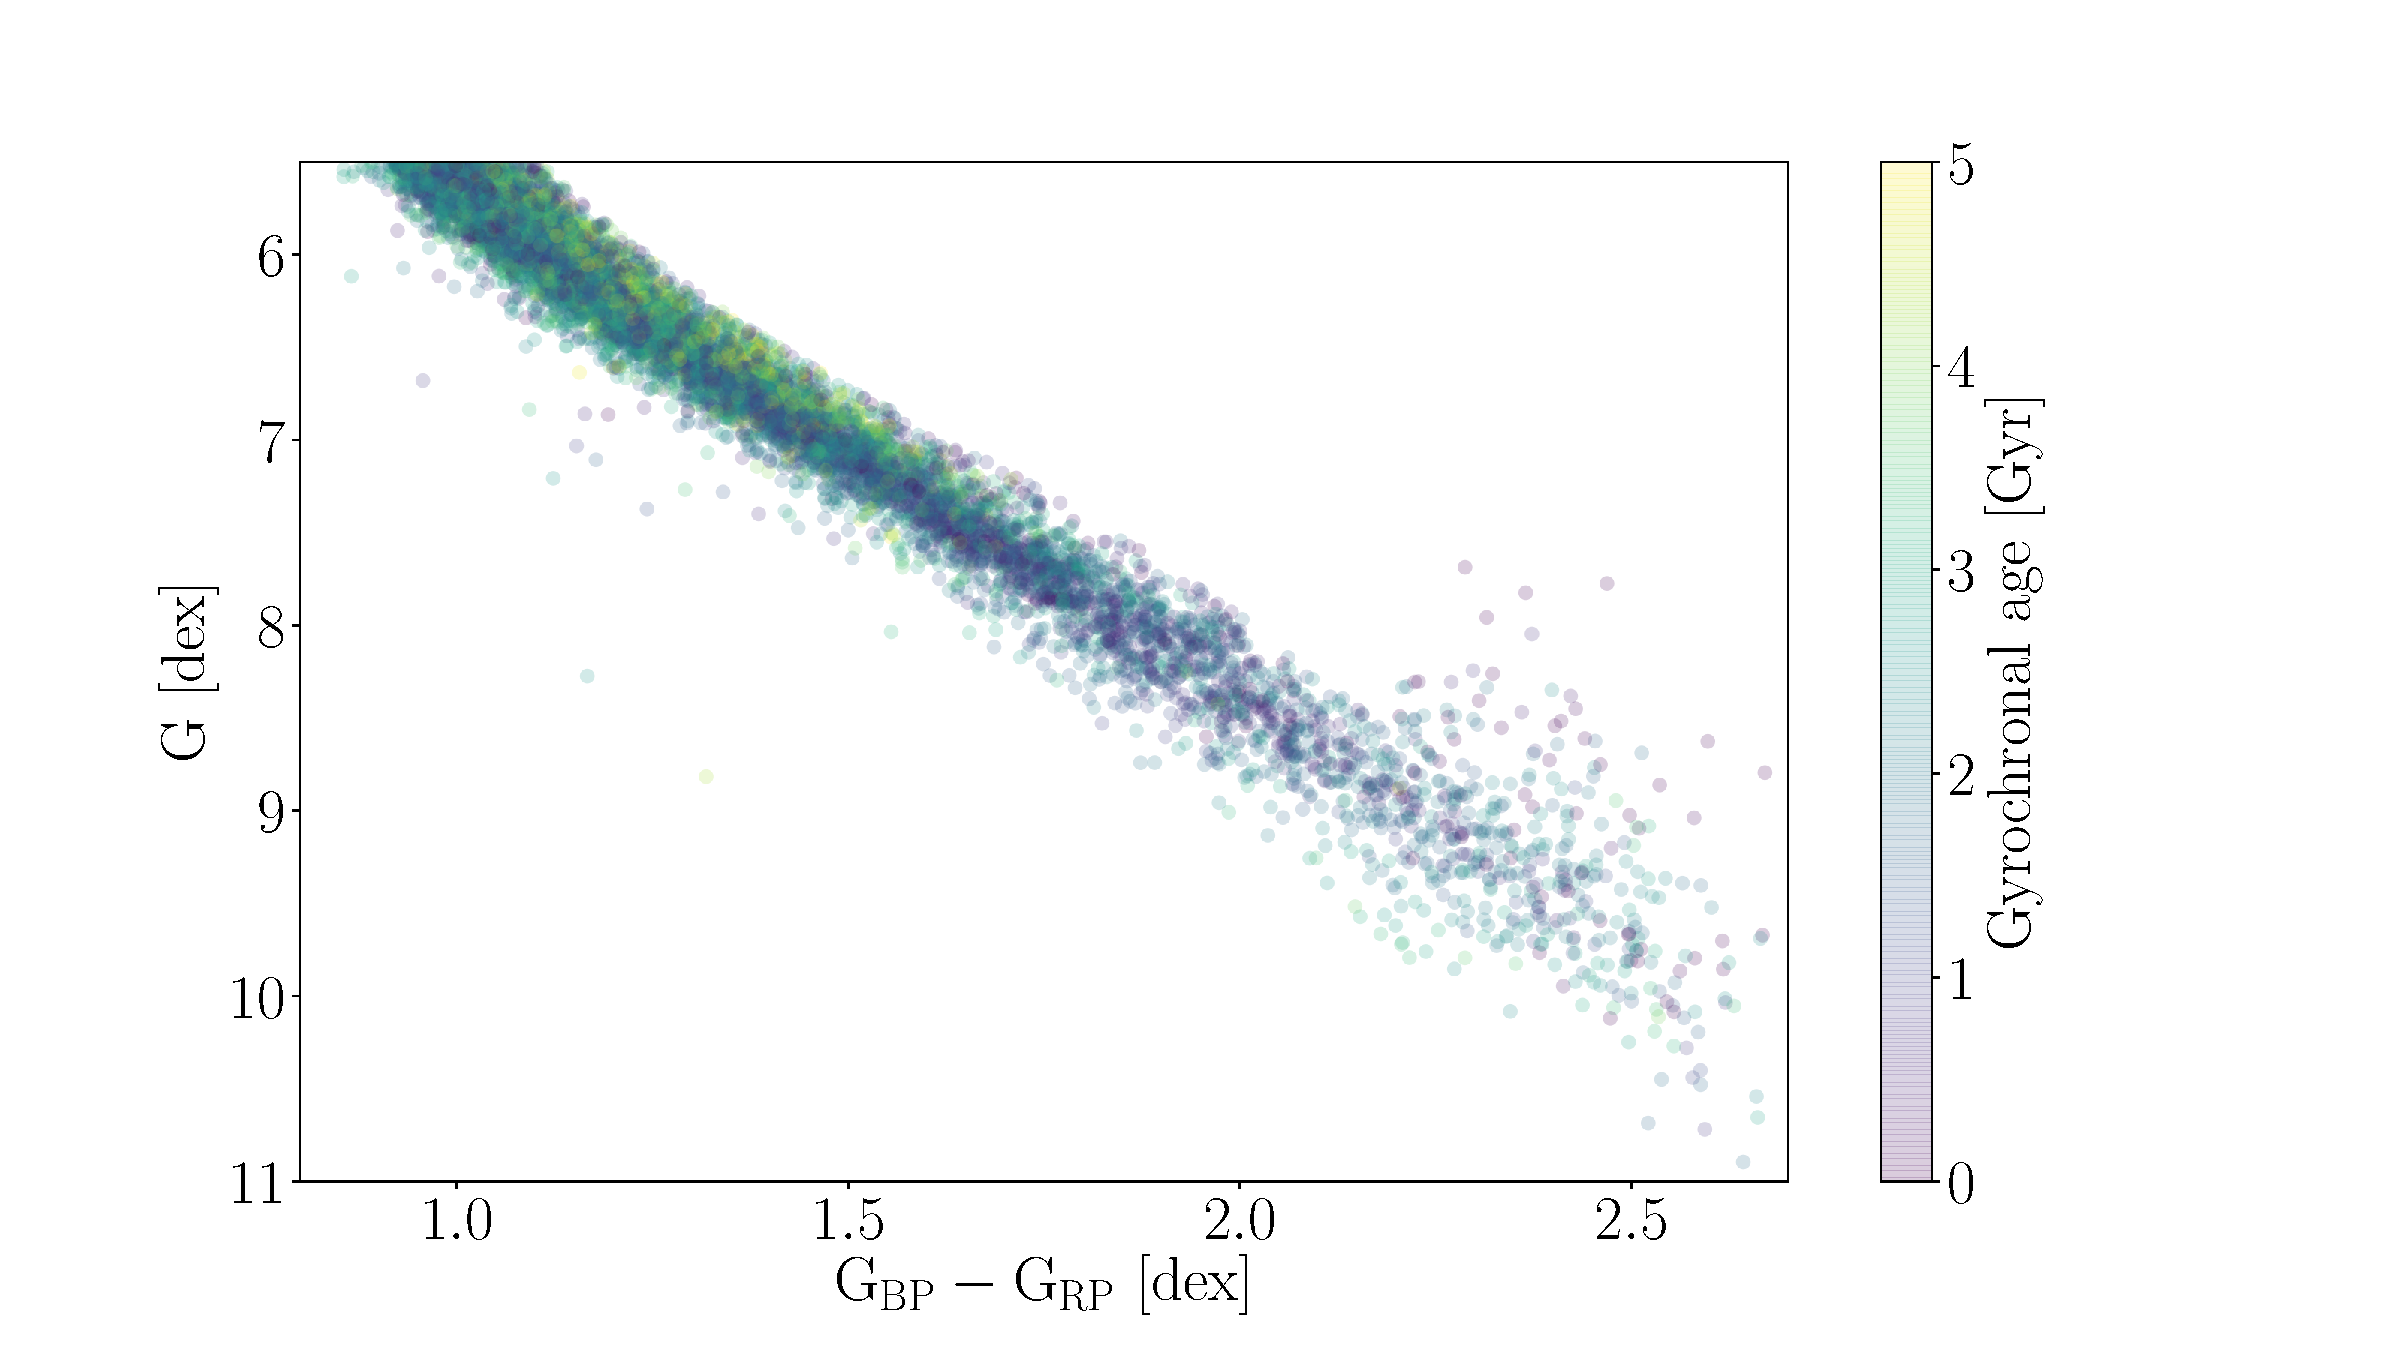
\includegraphics[width=1\textwidth]{age_gradient}
% \label{fig:age_gradient}
% \end{figure}
% Isochrones and stellar evolution tracks are highly dependent on choices made
% about input physics and assumptions and have often been calibrated using
% different types of stars.
% As a result, different sets of models can have very different shapes on the
% CMD, particularly at low masses.
% Instead of relying on CMD position to age-date groups of stars, we opted to
% explore age trends via kinematics.
% Kinematic age-dating has the advantage of being relatively model independent,
% or at least, having a very simple model: that velocity dispersion increases
% over time.
% This means that it is relatively easy to rank groups of stars by age: older
% groups have a larger velocity dispersion.
% It is less easy to rank-order groups of stars by age on the CMD because
% stellar evolution is highly mass and metallicity dependent, and because
% different stellar evolution models predict different ages for the same CMD
% position.
% This does not mean that it is not possible to calibrate gyrochronology using
% isochrones, however it is not the focus of this study.

% To examine the rotation period-temperature/color relation, we
% selected stars in the \mct\ sample with the same gyrochronal age, calculated
% using the \citet{angus2019} relations.
% Ages were calculated using dereddened \gaia\ \gcolor\, however we throughout
% this paper we show rotation periods as a function of effective temperature.

\begin{figure}
  \caption{
Top: rotation period vs effective temperature for stars in the \mct\
    catalog.
    The full catalog, with subgiants and visual binaries removed is shown in
    grey, and stars selected to be in different age groups are overlayed in
    color.
    These age groups were selected using the \citet{angus2019} gyrochronology
    relation.
The legend in the center of the figure lists the age range of each group.
    Bottom: velocity dispersion vs effective temperature for each age group.
The color of the line corresponds to the color of the group shown in the top
    panel.
If the gyrochronal model were correct at all ages and the stars in each group
    were the same age across temperatures, the velocity dispersion would be
    constant as a function of \teff.
However, the velocity dispersions of the oldest age groups depend on \teff,
    indicating that the \citet{angus2019} gyrochronology model either
    overpredicts the ages of old M dwarfs or underpredicts the ages of old G
    and K dwarfs.
}
  \centering
    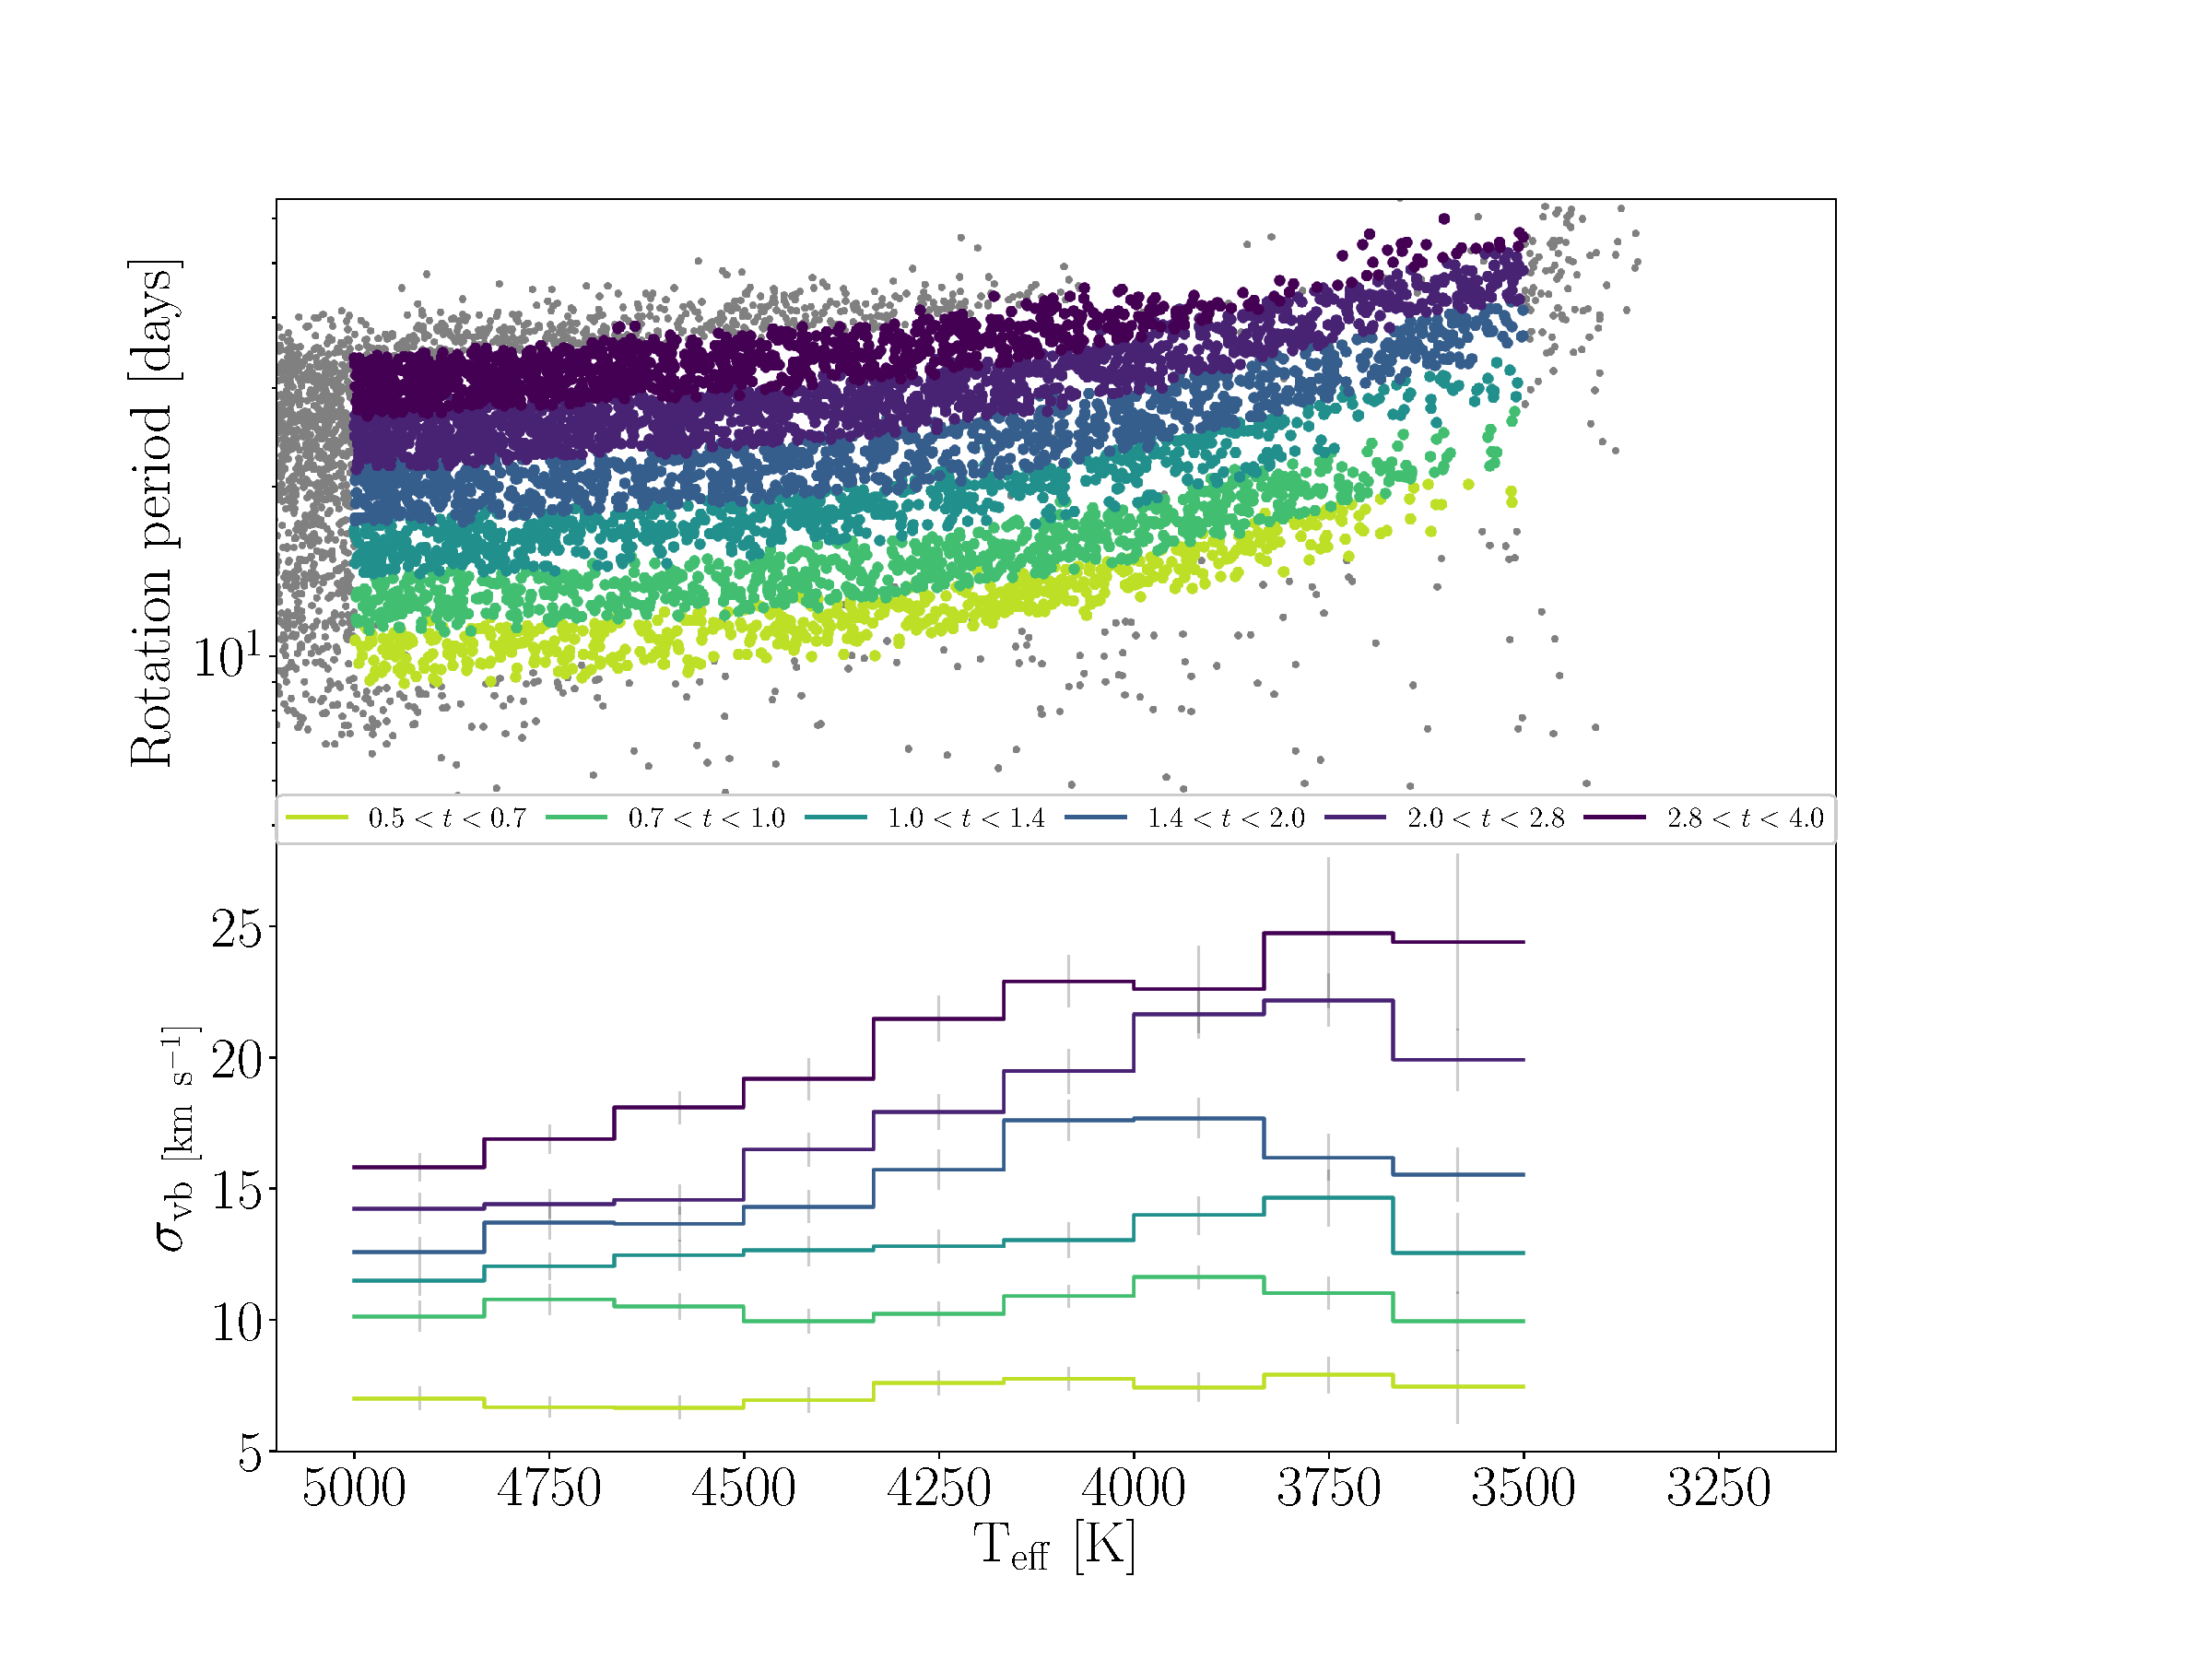
\includegraphics[width=1\textwidth]{age_cut}
\label{fig:age_cut}
\end{figure}
The top panel of figure \ref{fig:age_cut} shows the full \mct\ sample (minus
visual binaries and subgiants) in grey, with groups selected by age shown in
color.
The color of the points corresponds to the age ranges specified in the legend,
which also apply to the lines in the lower panel.
The bottom panel shows the velocity dispersion of each age group, as a
function of effective temperature.
We only included stars within a temperature range of 5000 - 3500 K in our
analysis, as hotter stars are more likely to have stopped magnetic braking
\citep{vansaders2016}, which could bias the results.
M dwarfs were not included in our analysis because such faint stars cannot be
observed at large heights above the plane (because of the low galactic
latitude of the \kepler\ field, stars at high-Z are more distant), which
introduces a mass-dependent velocity bias: cooler populations of stars are
skewed towards lower velocity dispersions.
The coolest temperature bins in figure \ref{fig:age_cut} have low velocity
dispersions, indicating that this effect may already become important at
temperatures lower than $\sim$ 4000 K.

Overall, figure \ref{fig:age_cut} shows that velocity dispersion increases
with gyrochronal age across all temperatures.
However, if the stars in each selected age group had the {\it same} age across
the temperature range, their velocity dispersion would be a constant function
of \teff.
Although the youngest age groups have a relatively constant velocity
dispersions across temperatures, the oldest age groups do not.
This indicates {\it either} that the shape of the period-color relation does
not remain constant over time, \ie\ it flattens out, {\it or} that cool stars
experience more efficient dynamical heating than hot stars.

Mass-dependent dynamical heating could occur because lower-mass stars
experience greater velocity changes when gravitationally perturbed.
However, mass-dependent orbital heating has not yet been unambiguously
observed in the galactic disk because of the strong anti-correlation between
stellar mass and stellar age.
Less massive stars do, indeed have larger velocity dispersions, however they
are also older on average.
This mass-age degeneracy is highly reduced in M dwarfs because their
main-sequence lifetimes are longer than the age of the Universe, however no
evidence for mass-dependent heating has been detected in these low mass stars
\citep{faherty2009}.

To investigate further, we calculated the exponent of the AVR for each
temperature bin in figure \ref{fig:age_cut}.
If mass-dependent heating is strongly affecting our data, the exponent of the
AVR should increase with decreasing effective temperature, \ie\ the heating
rate should be greater for lower-mass stars.
Figure \ref{fig:AVR_exponent} shows the AVR exponent does indeed increase with
decreasing effective temperature, however, the AVR exponent calculated using
more massive stars from the Geneva Copenhagen Survey (GCS)
\citep{holmberg2009} is also shown on this plot as a dashed horizontal line.
Most GCS stars are F and G type: 1-3 times more massive than the K dwarfs used
in our study.
If mass-dependent orbital heating is the main cause the rise in velocity
dispersion with decreasing \teff\ seen in figure \ref{fig:age_cut}, then the
AVR exponent of the more massive GCS stars should fall {\it below} the AVR
exponent for the most massive stars in our sample.
In other words, the dynamical heating rate should be lowest for the highest
mass stars and highest for the lowest mass stars.
\begin{figure}
  \caption{
The exponent of the AVR as a function of effective temperature.
    The AVR exponent of \citet{holmberg2009}, calculated using a more massive
    sample of stars, is shown as a horizontal dashed line.
}
  \centering
    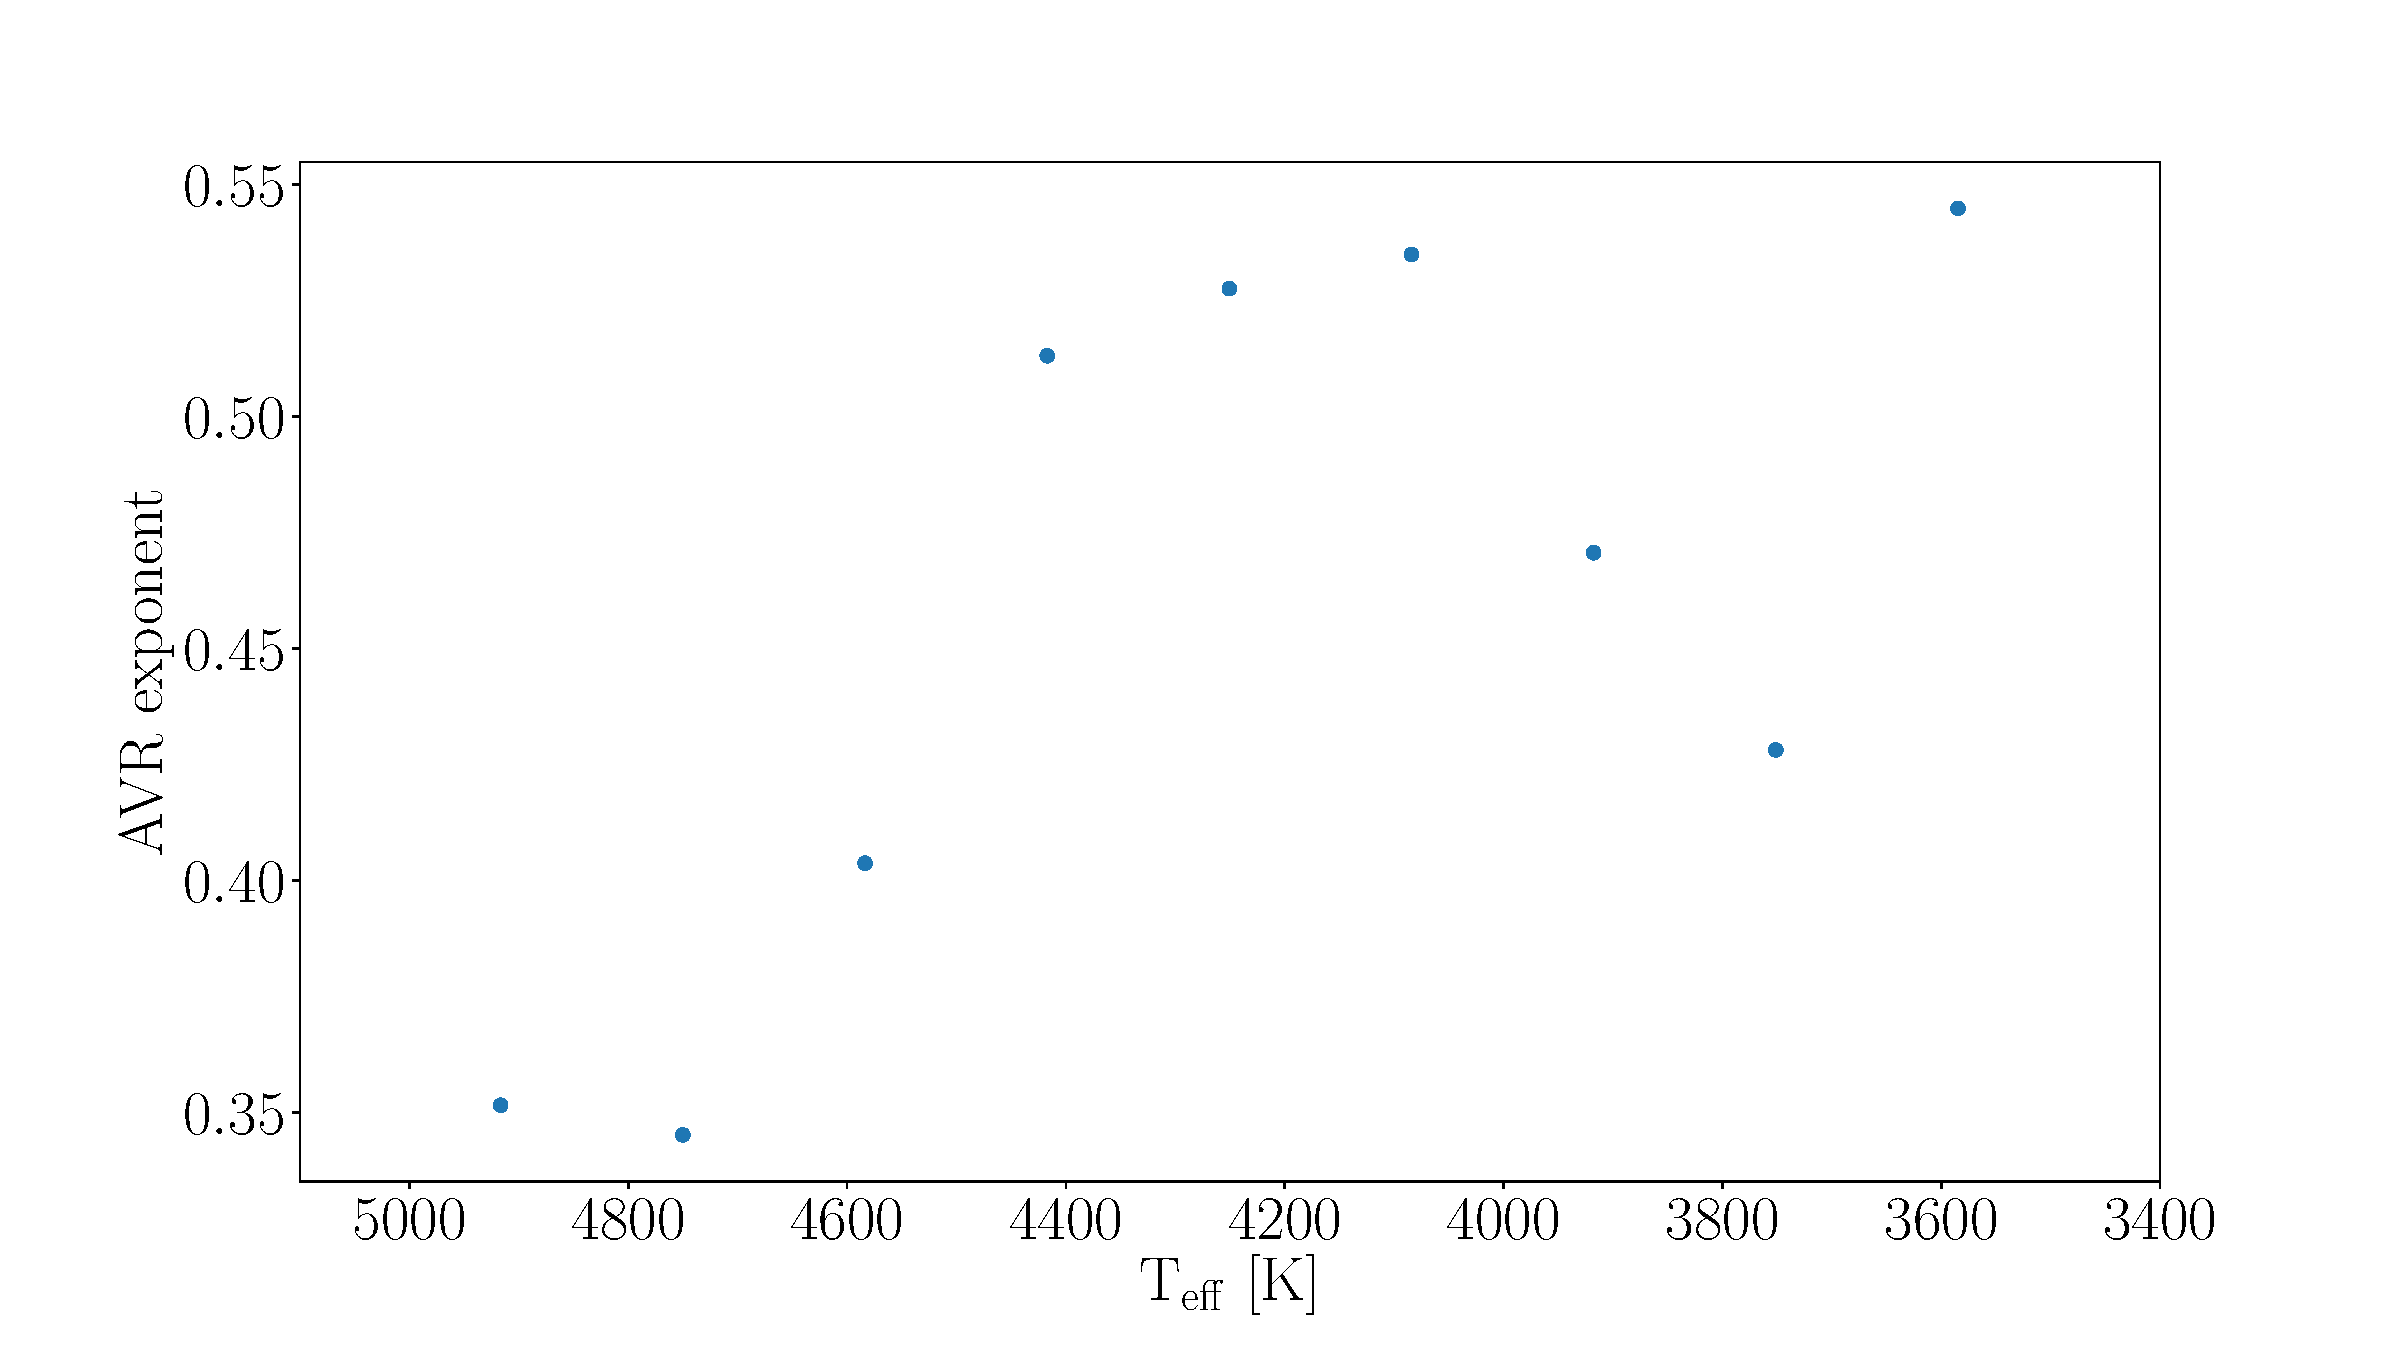
\includegraphics[width=1\textwidth]{AVR_exponent}
\label{fig:AVR_exponent}
\end{figure}
% nordstrom2004, jorgensen2005,
These AVR exponents were calculated with different populations of stars,
subject to different selection effects, so directly comparing them comes with
some risk.
The most important difference is that the GCS AVR is calculated using \vz,
however our AVRs are calculated using \vb\ since most stars in our sample do
not have radial velocities.
The median galactic latitude of these \kepler\ stars is 12.3\degrees, with
latitudes ranging from 5.5\degrees\ to 21.4\degrees, so \vb\ is a relatively
close approximation to \vz.
Only 290 out of the 6820 stars in our sample, plotted in color in figure
\ref{fig:age_cut}, have \gaia\ radial velocities, however we used the ones
that do to compare the \vz\ AVR to the \vb\ AVR, across all temperatures
between 3500 and 5000 K.
For stars with gyrochronal ages between 0.5 and 4.5 Gyr, we measured a \vz\
AVR exponent of 0.519 $\pm$ ... and a \vb\ AVR exponent of 0.514 $\pm$... .
The similarity of these two AVR exponents suggests that directly comparing
these two quantities {\it may} be a reasonable approach.
For now, given the large difference between the (\vz) AVR exponent of the GCS
sample and the (\vb) AVR exponent of the hottest stars in our sample, we
assume that the increased velocity dispersion at cooler temperatures is mostly
caused by incorrect age-grouping due to an incorrect period-color relation at
old ages, and that any mass-dependent heating, while it may contribute at a
low level to this result, is not the dominant driver.
However, differentiating the effects of mass-dependent heating and the shape
of the gyrochronology relations is certainly warranted in a follow-up study.

% We explore the differences between these two scenarios in section
% \ref{sec:discussion} and find that an incorrect period-color relation is more
% likely to be the cause of this effect than mass-dependent heating.

% In the oldest age group, the cool stars have a larger velocity dispersion than
% the hot stars, suggesting that the cool stars are older than the hot stars
% (\ie\ these stars do not actually belong in the same age group).
% The velocity dispersion of the early Ks show remarkable agreement with
% observations of $\sigma_W$ as a function of age from the Geneva-Copenhagen
% survey \citep{Holmwood2009}.
% This indicates that the ages of early K stars are correctly predicted by this
% gyrochronolgy relation but the ages of late Ks are under-predicted.
% Alternatively, the cause of the increased dispersion as a function of
% temperature could be mass-dependent dynamical heating, whereby less massive
% stars experience larger velocity kicks than more massive stars.
% We discuss the differences between these two scenarios in section
% \ref{sec:results}.

% Figure \ref{fig:AVR_exponent} shows that AVR of stars between around 4170 K
% and 4330 K most closely matches the GCS AVR.

The Praesepe-calibrated gyrochronology relation seems to accurately predict
the relative ages of {\it young} field stars.
This is shown by the consistent velocity dispersion of young stars as a
function of temperature in figure \ref{fig:age_cut}.
To our knowledge, no gyrochronology relation has never been demonstrated to
correctly predict ages (either relative or absolute) for such cool or such
young field stars.
This is not particularly remarkable however, since these young stars are a
similar age to the Praesepe cluster, which was used to calibrate the
period-color relation.
Figure \ref{fig:age_comparison} shows the ages of star groups, predicted with
the \citet{angus2019} gyrochronology relation, compared with the ages of star
groups, predicted with the \citet{holmberg2009} AVR.
\citet{holmberg2009} only provide an exponent (0.53), not an intercept, for the
relation between logarithmic age (in Gyr) and logarithmic, \vz\ velocity
dispersion (in \kms), so we fit the intercept to the mean \vb\ velocity
dispersion across all temperatures, of our sample.
\begin{figure}
  \caption{
      Ages predicted by the \citet{holmberg2009} \vz\ AVR, against ages
    predicted by the \citet{angus2019} gyrochronology relation, for stars in
    different temperature ranges.
Points are colored by the effective temperature in the center of the \teff\
bin.
The dashed line shows the y=x relation.
Predicted kinematic ages fan out over gyrochronal time, either because the AVR
    is temperature-dependent or because the gyrochronology relations have an
    age-dependent period-color relation.
}
  \centering
    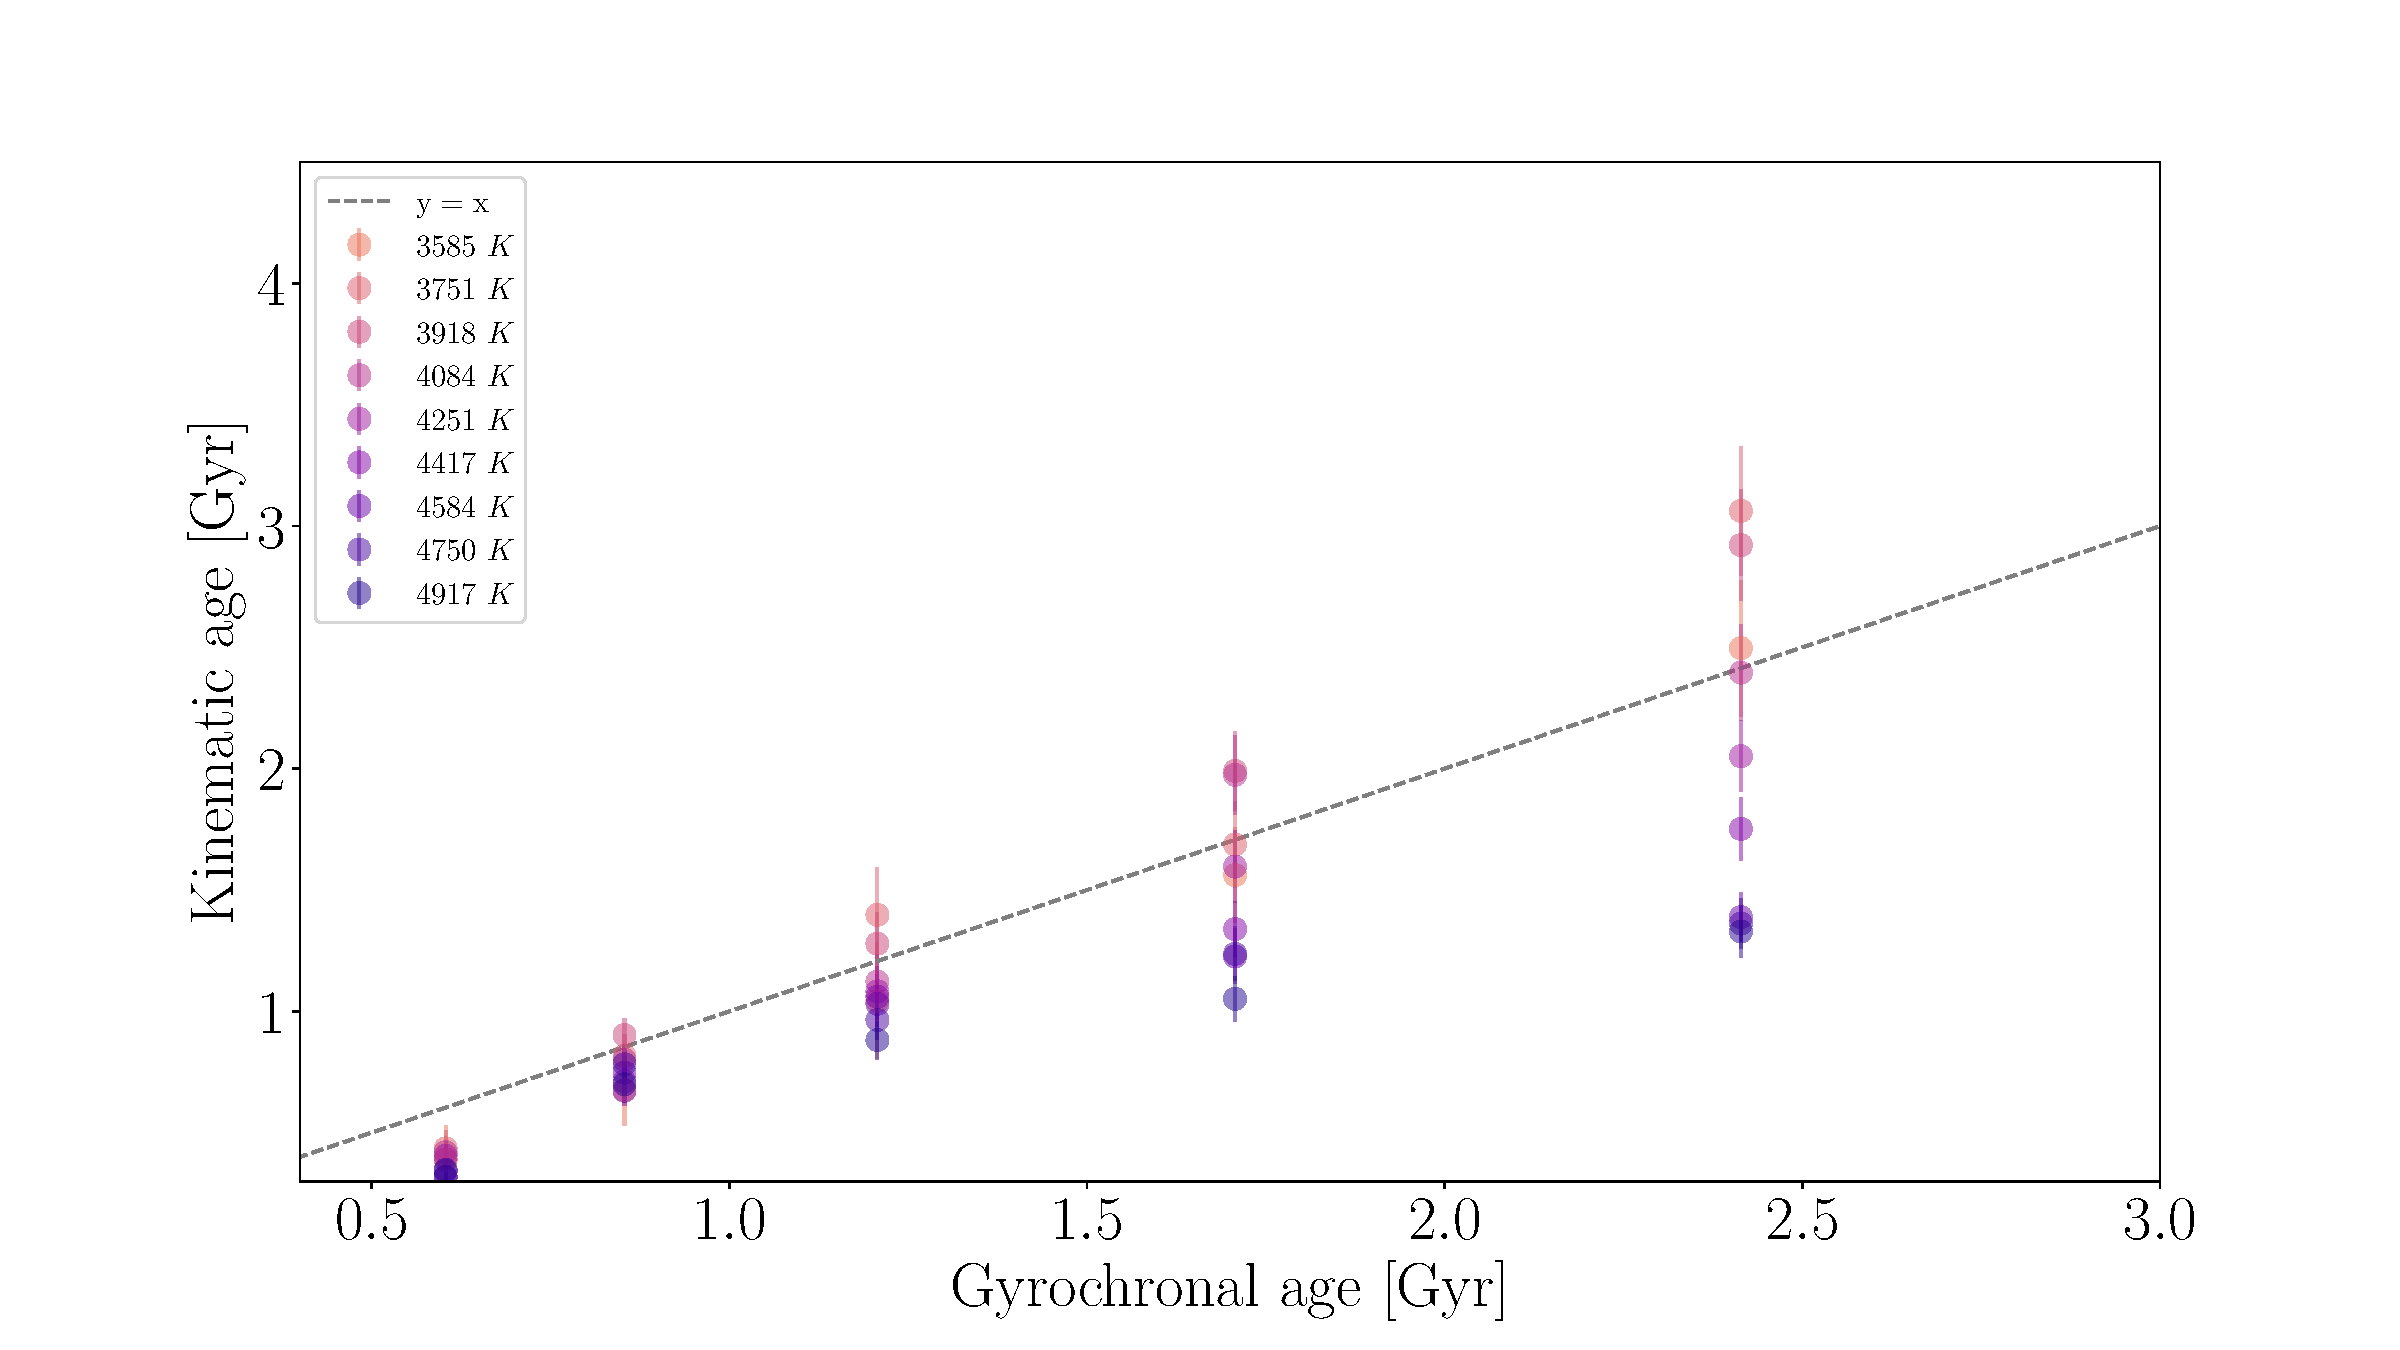
\includegraphics[width=1\textwidth]{age_comparison}
\label{fig:age_comparison}
\end{figure}
Figure \ref{fig:age_comparison} shows a comparison between ages predicted by
the \citet{holmberg2009} \vz\ AVR (using \vb\ as a proxy for \vz) and ages
predicted by the \citet{angus2019} gyrochronology relation, for stars in
different temperature ranges.
The predicted kinematic ages fan out over gyrochronal time, either because the
AVR is temperature-dependent or because the gyrochronology relations have an
age-dependent period-color relation.
Figure \ref{fig:age_comparion} also shows that the AVR seems to break down for
the youngest age bin, 0.5 Gyr, which has a lower velocity dispersion than
expected, given its age.
Alternatively, the ages of these young stars could be under-predicted by
gyrochronology.
These young stars have similar rotation periods to the Praesepe cluster, which
was used to calibrate the gyrochronology relation used in this analysis.
The ages of these young stars should, therefore, be the most accurate of the
entire sample.
However, they are tied to the age of the Praesepe cluster, whose age is not
accurately known.
\citet{angus2019} adopted an age for Praesepe of 650 Myrs, however the
kinematic age-prediction for these stars is around 400 Myrs.
Other studies have assigned a much older age of 800 Myrs to Praesepe
\citep{brandt2015}.
If the age assumed for Praesepe in the \citet{angus2019} gyrochronology
calibration was inaccurate, the entire age {\it scale} would be incorrect.
However, this is not what figure \ref{fig:age_comparion} shows -- it shows
that the {\it relative} age of these youngest stars are under-predicted by
kinematics or over-predicted by gyrochronology.

% Either the cool stars are being grouped into an age bin that is too young, or
% the hot stars are grouped into an age bin that is too old, but either way, the
% isochrones used to make the age selection are too steeply sloped.

We applied the same analysis described at the beginning of this section to
groups of stars selected using rotation period groups, instead of age groups.
The top panel of figure \ref{fig:period_cut} shows the \mct\ sample with
stars in different period ranges plotted in different colors.
The bottom panel shows the velocity dispersion of each group as a function of
effective temperature.
\begin{figure}
  \caption{
This figure is similar to figure \ref{fig:age_cut}, with stars divided into
    period groups rather than age groups.
The velocity dispersion is more constant across effective temperatures for the
    most slowly rotating stars, compared to the stars selected with the
    \citet{angus2018} gyrochronology model.
    This indicates that the gyrochronology models flatten out, and possibly
    even invert, at old ages.
}
  \centering
    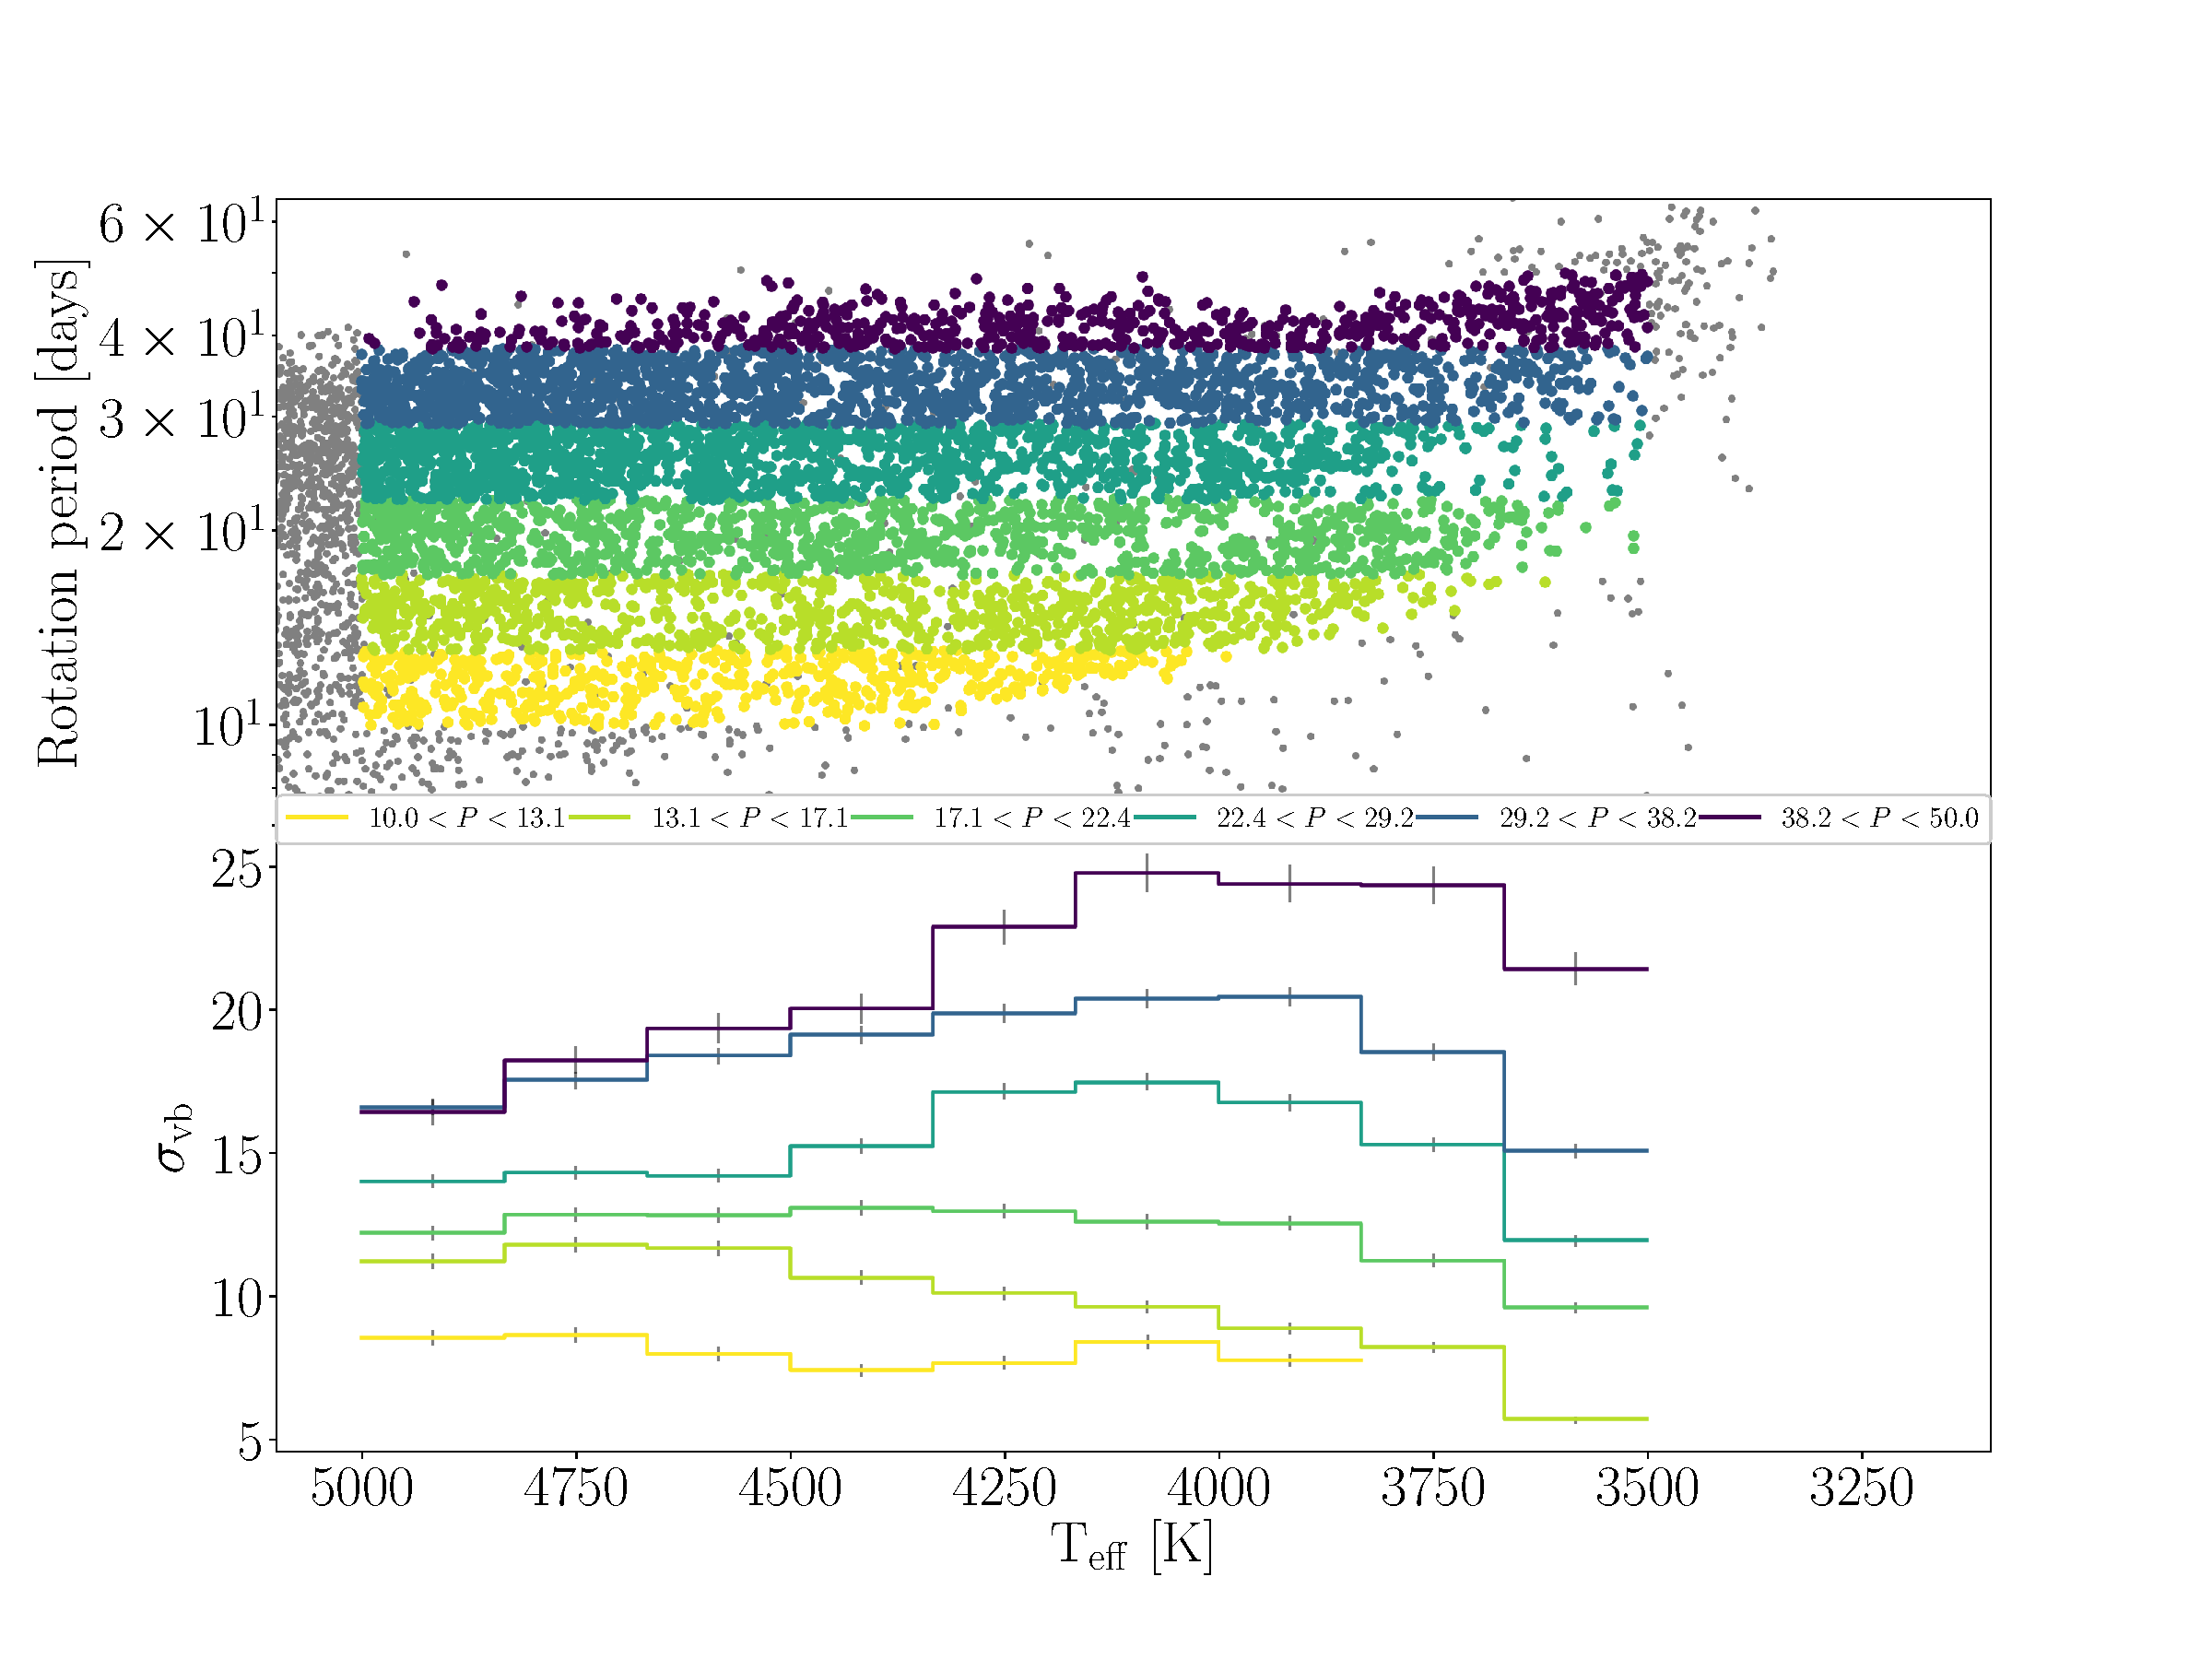
\includegraphics[width=1\textwidth]{period_cut}
\label{fig:period_cut}
\end{figure}
Once again, the velocity dispersion increases with rotation period overall.
For the most rapidly rotating groups of stars, velocity dispersion decreases
with \teff.
This is expected given the positively sloped period-color relation of Praesepe
and other young clusters: late K dwarfs rotate more slowly than early K dwarfs
of the same age.
Between 15 and 25 day rotation periods, the temperature dependence of the
velocity dispersion starts to disappear, indicating that the period-color
relation becomes flat: late K dwarfs rotate at the same rate as early K dwarfs
of the same age.
At long rotation periods, the velocity dispersion still increases with
effective temperature, although the increase is much more modest than in
figure \ref{fig:age_cut}.
This suggests that the period-color relation may have a negative slope at old
ages: late K dwarfs may rotate {\it more} rapidly than early K dwarfs.
This would be a paradigm shift for gyrochronology, since the assumption has
always been that stellar spin-down rate is tied to magnetic field strength.
The deeper convection zones of later type stars generate stronger magnetic
fields which {\it should} lead to more efficient angular momentum loss.

% \begin{figure}
%   \caption{
% Rotation period vs. velocity in the galactic latitute direction.
% }
%   \centering
%     \includegraphics[width=1\textwidth]{rotation_vb_dispersion}
% \label{fig:rotation_vb_dispersion}
% \end{figure}

% \begin{figure}
%   \caption{
% Age vs. velocity in the galactic latitute direction.
% The velocity of stars as a function of their age.
% }
%   \centering
%     \includegraphics[width=1\textwidth]{age_vb_dispersion}
% \label{fig:age_vb_dispersion}
% \end{figure}

% figure \ref{age_vb_dispersion} shows the velocity of stars in the \bvector\
% direction, plotted against their gyrochronal ages.
% These ages were calculated using equation 1 of \citet{stardate_paper},
% implemented in the \sd\ \python\ package \citep{stardate}.
% The two vertical lines show the approximate locations of the synchronized
% binary upper limit and the rotation gap.
% Stars to the left of the rotation gap (age $\lesssim$ 1 Gyr) and to the right
% of the synchronized binary regime (age $\gtrsim$ 0.5 Gyr) have lower $V_b$
% dispersion than stars to the right of the rotation gap (age $gtrsim$ 1 Gyr),
% indicating that they are kinematically young.
% This increase in velocity dispersion can be seen in both the individually
% plotted stars, and in the bins of standard deviation shown as the solid black
% line, which increase with age.
% This figure clearly indicates that stars with rotation periods that indicate
% they are young (but are greater than 7 days), are indeed young.
% This rules out the possibility that the rotation period gap is caused by
% either incorrect rotation periods, or binarity.

% This figure also shows a lack of M dwarfs at old ages caused by the `M dwarf
% dip' \citep{vansaders2019, mcquillan2014}.
% This is a feature of the \citet{mcquillan2014} sample where there appears to
% be a lack of slowly rotating stars at temperatures cooler than 4000 K.
% Like the rotation period gap, the origin of the M dwarf dip could either be
% due to a lack of stars with long rotation periods, or due to a suppression in
% the amplitudes of variability for these stars.
% However, in general the completeness of the \citet{mcquillan2014} catalog
% increases as a function of decreasing temperature, and is around 80\% for M
% dwarfs \citep{mcquillan2013, mcquillan2014, simonian2019}.
% This suggests that the age-rotation relation has a different shape at
% different ages, as indicated by the 1 Gyr NGC 6811 cluster that has a
% different rotation period-age relation to those of younger clusters
% \citep{curtis2019}.
